\subsection{Color Representation}

\begin{frame}{Light and color representation}
  \begin{minipage}[c]{0.75\textwidth}
    \begin{itemize}
    \item \textbf{Light} itself must be quantized in digital representations\\
    \textit{distinct from and unrelated to spatial quantization}
    \item Perceived as \textbf{colors} based on the Human visual system
      \begin{itemize}
      \item Perception based on \textbf{trichromacy} (red, green, blue)
      \item Not necessarily a unique frequency of the spectrum\\
      \textit{e.g. pink is not a color of the visible spectrum}
      \end{itemize}
    \item \textbf{Translating} light information (colors) to numbers:
      \begin{itemize}
      \item Colors are represented in a \textbf{tridimensional linear space}\\
      \textit{Grassmann’s laws approximation, generally using RGB}
      \item A \textbf{colorspace} defines a complete translation referential\\
      \textit{with specific primaries as a base and a white point}
      \item A triplet of values represents a \textbf{unique color} in a colorspace
      \item The \textbf{color gamut} is the range of colors in the colorspace\\
      \textit{not every color can be represented in every colorspace}
      \end{itemize}
    \end{itemize}
  \end{minipage}
  \hfill
  \begin{minipage}[c]{0.225\textwidth}
    \centering
    \includegraphics[width=\textwidth]{slides/graphics-theory-color/gamut.png}\\
    \textit{\small Color gamut of a given colorspace}
  \end{minipage}
\end{frame}

\begin{frame}{Color quantization approaches}
  \begin{minipage}[c]{0.75\textwidth}
  \begin{itemize}
    \item Different approaches exist for \textbf{color quantization}:
      \begin{itemize}
      \item \textbf{Uniform} quantization in the color range (most common)\\
        \textit{values are attributed to colors with a regular step (resolution)}
      \item \textbf{Irregular} quantization with indexed colors (palettes)\\
        \textit{values are attributed to colors as needed}
      \end{itemize}
    \item Uniform color coordinates are quantized with:
      \begin{itemize}
      \item A given \textbf{resolution}:
      \textit{the smallest possible color difference}
      \item A given \textbf{range}:
      \textit{the span of representable colors}
      \end{itemize}
    \item A given number of bits are used for quantization: \textbf{bit depth}
    \item A \textbf{trade-off} between range and resolution must be defined
      \begin{itemize}
      \item Increasing the resolution reduces the range
      \item Increasing the range reduces the resolution
      \end{itemize}
    \item A \textbf{transfer function} (EOTF/gamma) allows non-linear encoding
  \end{itemize}
  \end{minipage}
  \hfill
  \begin{minipage}[c]{0.225\textwidth}
    \centering
    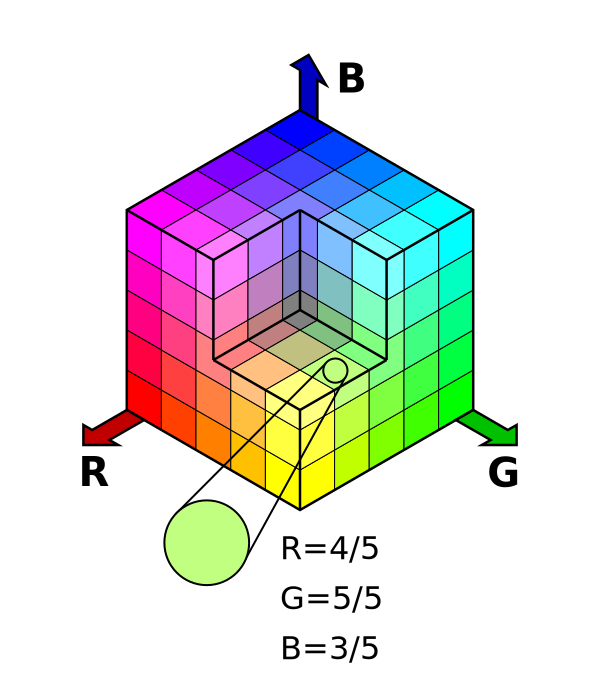
\includegraphics[width=\textwidth]{slides/graphics-theory-color/rgb-cube.pdf}
  \end{minipage}
\end{frame}

\begin{frame}{Light representation, color quantization (illustrated)}
  \begin{minipage}[b]{0.45\textwidth}
    \centering
    \includegraphics[width=\textwidth]{slides/graphics-theory-color/pair-of-merops.jpg}
  \end{minipage}
  \hfill
  \begin{minipage}[b]{0.45\textwidth}
    \centering
    \includegraphics[width=\textwidth]{slides/graphics-theory-color/pair-of-merops-16-colors.jpg}
  \end{minipage}

  \begin{center}
     \textit{\small A pair of Merops feeding}
  \end{center}

  \begin{minipage}[b]{0.45\textwidth}
    \centering
    \textbf{16 million colors (24 bits per pixel)}
    \begin{itemize}
    \item high color resolution
    \item high color range
    \end{itemize}
  \end{minipage}
  \hfill
  \begin{minipage}[b]{0.45\textwidth}
    \centering
    \textbf{16 colors (4 bits per pixel)}
    \begin{itemize}
    \item medium color resolution
    \item low color range
    \end{itemize}
  \end{minipage}
\end{frame}

\begin{frame}{Light representation, color quantization (illustrated)}
  \begin{minipage}[b]{0.45\textwidth}
    \centering
    \includegraphics[width=\textwidth]{slides/graphics-theory-color/pair-of-merops.jpg}
  \end{minipage}
  \hfill
  \begin{minipage}[b]{0.45\textwidth}
    \centering
    \includegraphics[width=\textwidth]{slides/graphics-theory-color/pair-of-merops-16-colors-range.jpg}
  \end{minipage}

  \begin{center}
     \textit{\small A pair of Merops feeding}
  \end{center}

  \begin{minipage}[b]{0.45\textwidth}
    \centering
    \textbf{16 million colors (24 bits per pixel)}
    \begin{itemize}
    \item low color resolution
    \item high color range
    \end{itemize}
  \end{minipage}
  \hfill
  \begin{minipage}[b]{0.45\textwidth}
    \centering
    \textbf{16 colors (4 bits per pixel)}
    \begin{itemize}
    \item low color resolution
    \item high color range
    \end{itemize}
  \end{minipage}
\end{frame}

\begin{frame}{Color transforms and channels}
  \begin{minipage}[b]{0.7\textwidth}
    \begin{itemize}
    \item Each component of a color triplet is called a \textbf{channel}
      \begin{itemize}
      \item RGB: \textbf{R} (red) / \textbf{G} (green) / \textbf{B} (blue)
      \end{itemize}
    \item Color transforms introduce different bases :
      \begin{itemize}
      \item HSV: \textbf{H} (hue) / \textbf{S} (saturation) / \textbf{V} (value)
      \item YCbCr/YUV: \textbf{Y} (luminance) / \textbf{Cb} / \textbf{Cr} (chrominance)
      \end{itemize}
    \end{itemize}
  \end{minipage}
  \hfill
  \begin{minipage}[b]{0.25\textwidth}
    \centering
    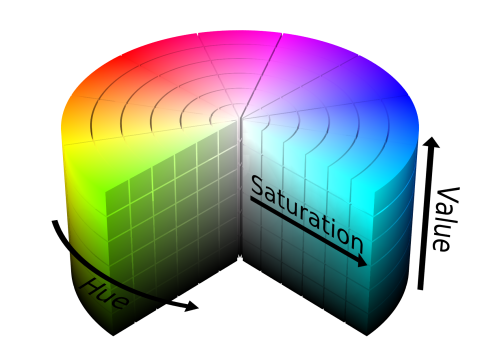
\includegraphics[width=\textwidth]{slides/graphics-theory-color/hsv-diagram.pdf}\\
    \vspace{-1em}
    \textit{\small HSV diagram}
    \vspace{0.25em}
  \end{minipage}
  \begin{itemize}
  \item An additional channel can exist for transparency: the \textbf{alpha channel}\\
  \textit{mostly relevant for composition, not for final display}
  \item Color triplets can be converted between representations:
    \begin{itemize}
    \item Between \textbf{color transforms} using given formulas (colorspace is preserved)
    \item Between \textbf{colorspaces} using constants and adaptation for limited gamuts
    \end{itemize}
  \end{itemize}
\end{frame}

\begin{frame}{Colorspaces and channels (illustrated with YUV)}
  \begin{minipage}[t]{0.25\textwidth}
    \centering
    \includegraphics[height=6em]{slides/graphics-theory-color/barn.jpg}\\
    \textit{\small Original picture}
  \end{minipage}
  \hfill
  \begin{minipage}[t]{0.7\textwidth}
    \centering
    \includegraphics[height=6em]{slides/graphics-theory-color/barn-yuv.jpg}\\
    \textit{\small Decomposition in Y, U and V channels}
  \end{minipage}

  \vspace{1em}

  \begin{minipage}[t]{0.4\textwidth}
    \small
    \begin{equation*}
    \begin{cases}
    R = Y + 1.140 \times V\\
    G = Y - 0.395 \times U - 0.581 \times V\\
    B = Y + 2.032 \times U
    \end{cases}
    \end{equation*}
  \end{minipage}
  \hfill
  \begin{minipage}[t]{0.55\textwidth}
    \small
    \begin{equation*}
    \begin{cases}
    Y = + 0.299 \times R + 0.587 \times G + 0.114 \times B\\
    U = - 0.147 \times R - 0.289 \times G + 0.436 \times B\\
    V = + 0.615 \times R - 0.515 \times G - 0.100 \times B
    \end{cases}
    \end{equation*}
  \end{minipage}

  \begin{center}
     \textit{\small Translation between BT.601 in YUV and sRGB in RGB}
  \end{center}
\end{frame}
